% Options for packages loaded elsewhere
\PassOptionsToPackage{unicode}{hyperref}
\PassOptionsToPackage{hyphens}{url}
\PassOptionsToPackage{dvipsnames,svgnames,x11names}{xcolor}
\documentclass[
  american,
  11pt,
]{article}
\usepackage{xcolor}
\usepackage[margin=1in]{geometry}
\usepackage{amsmath,amssymb}
\setcounter{secnumdepth}{-\maxdimen} % remove section numbering
\usepackage{iftex}
\ifPDFTeX
  \usepackage[T1]{fontenc}
  \usepackage[utf8]{inputenc}
  \usepackage{textcomp} % provide euro and other symbols
\else % if luatex or xetex
  \usepackage{unicode-math} % this also loads fontspec
  \defaultfontfeatures{Scale=MatchLowercase}
  \defaultfontfeatures[\rmfamily]{Ligatures=TeX,Scale=1}
\fi
\usepackage{lmodern}
\ifPDFTeX\else
  % xetex/luatex font selection
\fi
% Use upquote if available, for straight quotes in verbatim environments
\IfFileExists{upquote.sty}{\usepackage{upquote}}{}
\IfFileExists{microtype.sty}{% use microtype if available
  \usepackage[]{microtype}
  \UseMicrotypeSet[protrusion]{basicmath} % disable protrusion for tt fonts
}{}
\makeatletter
\@ifundefined{KOMAClassName}{% if non-KOMA class
  \IfFileExists{parskip.sty}{%
    \usepackage{parskip}
  }{% else
    \setlength{\parindent}{0pt}
    \setlength{\parskip}{6pt plus 2pt minus 1pt}}
}{% if KOMA class
  \KOMAoptions{parskip=half}}
\makeatother
\usepackage{longtable,booktabs,array}
\newcounter{none} % for unnumbered tables
\usepackage{calc} % for calculating minipage widths
% Correct order of tables after \paragraph or \subparagraph
\usepackage{etoolbox}
\makeatletter
\patchcmd\longtable{\par}{\if@noskipsec\mbox{}\fi\par}{}{}
\makeatother
% Allow footnotes in longtable head/foot
\IfFileExists{footnotehyper.sty}{\usepackage{footnotehyper}}{\usepackage{footnote}}
\makesavenoteenv{longtable}
\usepackage{graphicx}
\makeatletter
\newsavebox\pandoc@box
\newcommand*\pandocbounded[1]{% scales image to fit in text height/width
  \sbox\pandoc@box{#1}%
  \Gscale@div\@tempa{\textheight}{\dimexpr\ht\pandoc@box+\dp\pandoc@box\relax}%
  \Gscale@div\@tempb{\linewidth}{\wd\pandoc@box}%
  \ifdim\@tempb\p@<\@tempa\p@\let\@tempa\@tempb\fi% select the smaller of both
  \ifdim\@tempa\p@<\p@\scalebox{\@tempa}{\usebox\pandoc@box}%
  \else\usebox{\pandoc@box}%
  \fi%
}
% Set default figure placement to htbp
\def\fps@figure{htbp}
\makeatother
% definitions for citeproc citations
\NewDocumentCommand\citeproctext{}{}
\NewDocumentCommand\citeproc{mm}{%
  \begingroup\def\citeproctext{#2}\cite{#1}\endgroup}
\makeatletter
 % allow citations to break across lines
 \let\@cite@ofmt\@firstofone
 % avoid brackets around text for \cite:
 \def\@biblabel#1{}
 \def\@cite#1#2{{#1\if@tempswa , #2\fi}}
\makeatother
\newlength{\cslhangindent}
\setlength{\cslhangindent}{1.5em}
\newlength{\csllabelwidth}
\setlength{\csllabelwidth}{3em}
\newenvironment{CSLReferences}[2] % #1 hanging-indent, #2 entry-spacing
 {\begin{list}{}{%
  \setlength{\itemindent}{0pt}
  \setlength{\leftmargin}{0pt}
  \setlength{\parsep}{0pt}
  % turn on hanging indent if param 1 is 1
  \ifodd #1
   \setlength{\leftmargin}{\cslhangindent}
   \setlength{\itemindent}{-1\cslhangindent}
  \fi
  % set entry spacing
  \setlength{\itemsep}{#2\baselineskip}}}
 {\end{list}}
\usepackage{calc}
\newcommand{\CSLBlock}[1]{\hfill\break\parbox[t]{\linewidth}{\strut\ignorespaces#1\strut}}
\newcommand{\CSLLeftMargin}[1]{\parbox[t]{\csllabelwidth}{\strut#1\strut}}
\newcommand{\CSLRightInline}[1]{\parbox[t]{\linewidth - \csllabelwidth}{\strut#1\strut}}
\newcommand{\CSLIndent}[1]{\hspace{\cslhangindent}#1}
\ifLuaTeX
\usepackage[bidi=basic,shorthands=off]{babel}
\else
\usepackage[bidi=default,shorthands=off]{babel}
\fi
\ifLuaTeX
  \usepackage{selnolig} % disable illegal ligatures
\fi
\setlength{\emergencystretch}{3em} % prevent overfull lines
\providecommand{\tightlist}{%
  \setlength{\itemsep}{0pt}\setlength{\parskip}{0pt}}
\usepackage{bookmark}
\IfFileExists{xurl.sty}{\usepackage{xurl}}{} % add URL line breaks if available
\urlstyle{same}
\hypersetup{
  pdftitle={Curated resistance gene families outperform Evo 2 embeddings on unseen variants in Escherichia coli},
  pdfauthor={Rushath Rajeev},
  pdflang={en-US},
  colorlinks=true,
  linkcolor={Maroon},
  filecolor={Maroon},
  citecolor={Blue},
  urlcolor={Blue},
  pdfcreator={LaTeX via pandoc}}

\title{Curated resistance gene families outperform Evo 2 embeddings on
unseen variants in Escherichia coli}
\author{Rushath Rajeev}
\date{Preprint --- 3 October 2026}

\begin{document}
\maketitle
\begin{abstract}
Genomic foundation models may encode resistance-related sequence
variation beyond curated gene catalogues, but their value depends on
comparisons with appropriate biological baselines. We evaluated frozen
Evo 2 embeddings and AMRFinderPlus features for predicting minimum
inhibitory concentrations (MICs) of ceftriaxone, ciprofloxacin, and
gentamicin in Escherichia coli. The curated cohort contained 29,619
isolate--antibiotic measurements from 11,520 isolates, including 3,849
human-clinical development isolates and 1,505 external Japanese
isolates. We fitted regression models that account for censored MICs,
used nested cross-validation grouped by lineage, and froze external
predictions before accessing reference MICs. Evo 2 embeddings alone
performed worse than allele-level catalogue features for all three drugs
and both learners in the locked external evaluation. Adding embeddings
did not meet the prespecified criterion for improvement; a gentamicin
gain in development was specific to one source and reversed externally.
An exploratory external analysis found that curated gene-family and
drug-class features placed 99.0\% of 102 highly resistant carriers of
variants absent or nearly absent from development above a descriptive
ceftriaxone threshold, compared with 78.4--81.4\% for Evo 2 alone and
12.7--14.7\% for allele-level models. In a subsequent experiment
withholding four CTX-M alleles from development training, curated
features exceeded Evo 2 by 4.6 percentage points with regularized
regression (95\% lineage-bootstrap interval 2.3--12.1) and 11.1 points
with XGBoost (7.4--22.1). These findings favor curated biological
grouping over the tested embedding representation. Heterogeneous
development assays and reuse of external data for the exploratory
analysis limit generalization; the family-model result has not been
confirmed in a new external cohort.
\end{abstract}

\textbf{Affiliation:} Independent researcher.\\
\textbf{Correspondence:}
\href{mailto:rushathrajeevav@gmail.com}{\nolinkurl{rushathrajeevav@gmail.com}}

\section{Introduction}\label{introduction}

Whole-genome sequencing offers a route to predicting antimicrobial
resistance while identifying the genetic determinants associated with a
phenotype. In \emph{Escherichia coli}, models using gene content and
sequence variation have predicted resistance across multiple antibiotics
(\citeproc{ref-moradigaravand2018}{Moradigaravand et al. 2018}). Curated
resources such as AMRFinderPlus provide a complementary representation:
acquired resistance genes and selected mutations are identified using
accumulated experimental knowledge
(\citeproc{ref-feldgarden2021}{Feldgarden et al. 2021}). A useful new
representation should therefore be compared with strong implementations
of this existing knowledge.

Genomic foundation models provide an alternative way to represent
sequence. Evo 2 learns from a large collection of genomic sequences and
supports downstream prediction using its internal representations
(\citeproc{ref-brixi2026}{{Brixi et al.} 2026}). Such representations
could capture relationships between related resistance alleles or local
sequence context that a binary gene-name feature misses. Whether this
improves antibiotic susceptibility prediction is an empirical question.
In particular, a model can appear to improve when it recognizes lineages
or collection sources associated with a phenotype. Population structure
and biased sampling can confound genomic resistance prediction even in
large datasets (\citeproc{ref-yu2025}{Yu et al. 2025}).

The comparison also depends on how curated knowledge is encoded. A
predictor using a separate feature for each allele cannot directly
transfer a learned coefficient to an allele excluded from its training
vocabulary. A feature representing a gene family or drug class can
retain that connection. Comparing a sequence model only with an
allele-level catalogue may therefore attribute to representation
learning an advantage that a simple biological grouping supplies.

We tested whether Evo 2 representations improve prediction of
quantitative susceptibility to ceftriaxone, ciprofloxacin, and
gentamicin beyond AMRFinderPlus features. We first conducted development
analyses and one locked external evaluation using a Japanese
surveillance collection with standardized susceptibility testing
(\citeproc{ref-kayama2023}{Kayama et al. 2023}). We then investigated an
external failure involving resistance variants absent from development,
compared curated hierarchical features with Evo 2, and tested the
resulting hypothesis by withholding entire resistance alleles from
development training. The study distinguishes the original locked
evaluation, the exploratory external follow-up, and the subsequent
controlled development experiment.

\section{Results}\label{results}

\subsection{A quantitative cohort with an independent external
collection}\label{a-quantitative-cohort-with-an-independent-external-collection}

The final cohort contained 29,619 isolate--antibiotic rows from 11,520
isolates. Development data comprised 10,015 isolates from NCBI sources;
the primary training population was the 3,849 isolates identified as
human clinical using source metadata. Models trained on all development
sources formed a sensitivity analysis. The final external set contained
1,505 JARBS isolates with measurements for all three antibiotics (Table
1).

\textbf{Table 1. Final modelling cohort.} Drug columns count reconciled
isolate--antibiotic MIC rows. Human-clinical development is a subset of
all-source development. External isolates are human clinical by the
source study design.

{\def\LTcaptype{none} % do not increment counter
\begin{longtable}[]{@{}lrrrr@{}}
\toprule\noalign{}
Population & Isolates & Ceftriaxone & Ciprofloxacin & Gentamicin \\
\midrule\noalign{}
\endhead
\bottomrule\noalign{}
\endlastfoot
Development, all sources & 10,015 & 7,097 & 8,493 & 9,514 \\
Development, human clinical & 3,849 & 2,822 & 3,809 & 3,348 \\
External, Japan & 1,505 & 1,505 & 1,505 & 1,505 \\
\end{longtable}
}

External exclusion used a sequence-based putative-duplicate rule fixed
before external modelling. Shared lineages were permitted; isolates
meeting the duplicate threshold against development were excluded. The
final external population contained 106 lineage groups, including 18
groups absent from development. Within development, the cross-validation
unit combined lineage, genomic cluster, and identifier-based duplicate
membership, producing 485 units.

Development susceptibility measurements came from heterogeneous sources
whose assay methods and testing dates were not consistently available.
In the initial development MIC snapshot, 18,136 of 25,466 rows (71.2\%)
were reported as bounds. We retained that censoring in model fitting and
scoring. The external collection used centralized broth microdilution,
but was enriched for resistance and was further selected by genomic
exclusion. It consequently measures transfer to this particular
challenge population rather than routine clinical performance.

\subsection{Evo 2 did not improve the locked external
benchmark}\label{evo-2-did-not-improve-the-locked-external-benchmark}

We compared two learners---regularized interval-censored regression,
abbreviated ridge, and XGBoost with an accelerated failure time
objective---using allele-level AMRFinderPlus features, Evo 2 embeddings,
or their concatenation. Constant-MIC and nearest-development-relative
predictors supplied reference baselines. Essential agreement (EA)
measured whether the predicted dilution was within one doubling step of
the reference value or the set allowed by a reported bound.

In human-clinical development, adding Evo 2 improved gentamicin EA for
both learners: the paired difference was 0.027 (95\% interval
0.010--0.038) for ridge and 0.024 (0.001--0.043) for XGBoost.
Ceftriaxone improved only with ridge, and ciprofloxacin showed no
demonstrated gain. The rule for crediting an Evo 2 improvement required
a positive paired interval for both learners in development and the
locked external evaluation. This rule was adopted after the
human-clinical development results were available, but before the
all-source Evo 2 results and before external outcomes were inspected.

The gentamicin gain was source-specific. Removing evaluation rows from
BioProject PRJNA1297298 changed the paired improvement to \ensuremath{-}0.001 (\ensuremath{-}0.006
to 0.002) for ridge and \ensuremath{-}0.002 (\ensuremath{-}0.008 to 0.002) for XGBoost. These were
analyses of existing out-of-fold predictions, not models retrained with
that source removed. The pattern is consistent with a contribution from
source-associated measurement conventions; it does not establish the
precise information encoded in the embeddings.

After external predictions were frozen, the gentamicin improvement
reversed: adding Evo 2 changed EA by \ensuremath{-}0.033 (\ensuremath{-}0.056 to \ensuremath{-}0.015) for ridge
and \ensuremath{-}0.021 (\ensuremath{-}0.046 to 0.000) for XGBoost (Figure 1). No drug met the
full improvement rule. Evo 2 features alone had lower external EA than
allele-level AMRFinderPlus features for every drug and learner. The
combined feature set also failed to demonstrate a consistent advantage.

\begin{figure}
\centering
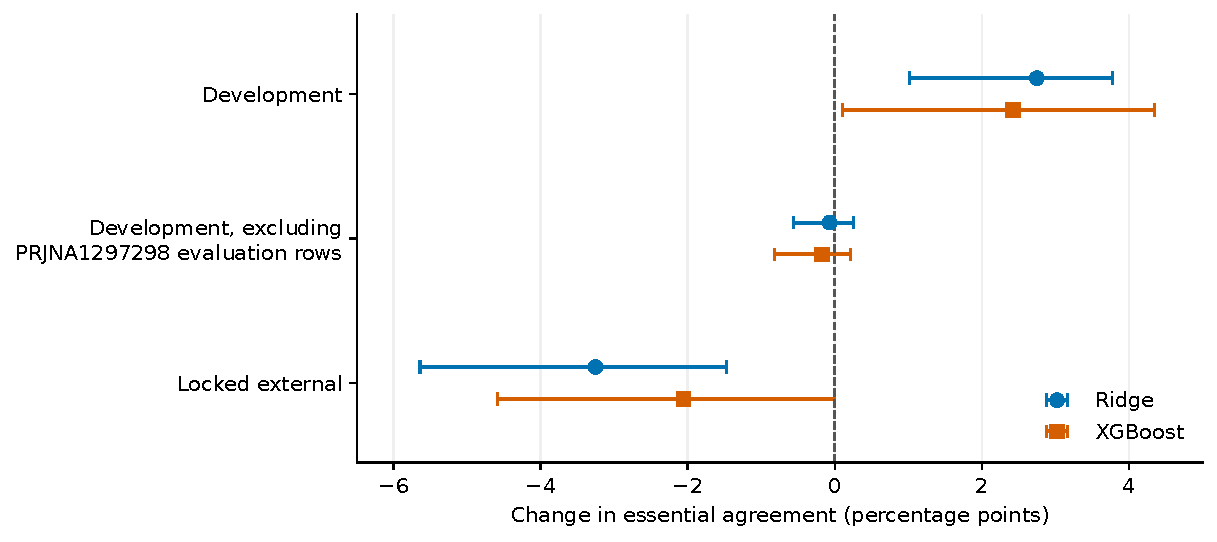
\includegraphics[width=0.95\linewidth,height=\textheight,keepaspectratio,alt={Figure 1. The gentamicin embedding gain depends on the evaluation population. Points show EA differences for AMRFinderPlus plus Evo 2 minus AMRFinderPlus alone; bars are reported 95\% paired lineage-bootstrap intervals. The middle comparison excludes PRJNA1297298 evaluation rows from existing development predictions and does not represent retraining without that source. External predictions were locked before reference MICs were read.}]{figures/figure1_gentamicin_gain.pdf}
\caption{The gentamicin embedding gain depends on the
evaluation population. Points show EA differences for AMRFinderPlus plus
Evo 2 minus AMRFinderPlus alone; bars are reported 95\% paired
lineage-bootstrap intervals. The middle comparison excludes PRJNA1297298
evaluation rows from existing development predictions and does not
represent retraining without that source. External predictions were
locked before reference MICs were read.}
\end{figure}

Allele-level catalogue models nevertheless transferred useful predictive
information (Table 2). External ciprofloxacin EA was 0.932 for ridge and
0.933 for XGBoost; gentamicin EA was 0.887 and 0.876. Ceftriaxone was
less accurate, with EA of 0.680 and 0.597. Each catalogue model exceeded
the constant baseline with a paired interval excluding zero. Ceftriaxone
had been labelled underpowered under the study's prespecified
interval-width criterion before external scoring.

\textbf{Table 2. Locked external results for allele-level AMRFinderPlus
features.} Training used human-clinical development isolates. Brackets
give 95\% lineage-bootstrap intervals. Under-call is the proportion of
right-censored references predicted at least two dilutions below the
allowed reference set; it is a quantitative MIC error measure.

{\def\LTcaptype{none} % do not increment counter
\begin{longtable}[]{@{}
  >{\raggedright\arraybackslash}p{(\linewidth - 6\tabcolsep) * \real{0.2500}}
  >{\raggedright\arraybackslash}p{(\linewidth - 6\tabcolsep) * \real{0.2500}}
  >{\raggedright\arraybackslash}p{(\linewidth - 6\tabcolsep) * \real{0.2500}}
  >{\raggedright\arraybackslash}p{(\linewidth - 6\tabcolsep) * \real{0.2500}}@{}}
\toprule\noalign{}
\begin{minipage}[b]{\linewidth}\raggedright
Drug
\end{minipage} & \begin{minipage}[b]{\linewidth}\raggedright
Learner
\end{minipage} & \begin{minipage}[b]{\linewidth}\raggedright
Essential agreement
\end{minipage} & \begin{minipage}[b]{\linewidth}\raggedright
Right-censored under-call
\end{minipage} \\
\midrule\noalign{}
\endhead
\bottomrule\noalign{}
\endlastfoot
Ceftriaxone & Ridge & 0.680 {[}0.539, 0.742{]} & 0.258 {[}0.181,
0.480{]} \\
Ceftriaxone & XGBoost & 0.597 {[}0.480, 0.692{]} & 0.513 {[}0.460,
0.669{]} \\
Ciprofloxacin & Ridge & 0.932 {[}0.894, 0.950{]} & 0.012 {[}0.003,
0.026{]} \\
Ciprofloxacin & XGBoost & 0.933 {[}0.913, 0.954{]} & 0.025 {[}0.013,
0.064{]} \\
Gentamicin & Ridge & 0.887 {[}0.841, 0.916{]} & 0.057 {[}0.031,
0.135{]} \\
Gentamicin & XGBoost & 0.876 {[}0.829, 0.909{]} & 0.121 {[}0.071,
0.269{]} \\
\end{longtable}
}

\textbf{Table 3. Complete primary locked external comparison.} Essential
agreement for models trained on human-clinical development data and
evaluated on the same 1,505 external isolates per drug. Full 95\%
intervals, exact-reference scores, and all-source training results are
provided in Supplementary Table S1. The post-hoc family models are
reported separately.

{\def\LTcaptype{none} % do not increment counter
\begin{longtable}[]{@{}lrrr@{}}
\toprule\noalign{}
Model & Ceftriaxone & Ciprofloxacin & Gentamicin \\
\midrule\noalign{}
\endhead
\bottomrule\noalign{}
\endlastfoot
Constant & 0.290 & 0.400 & 0.783 \\
Nearest relative & 0.529 & 0.849 & 0.752 \\
Ridge: allele & 0.680 & 0.932 & 0.887 \\
Ridge: Evo 2 & 0.579 & 0.870 & 0.822 \\
Ridge: allele + Evo 2 & 0.684 & 0.908 & 0.854 \\
XGBoost: allele & 0.597 & 0.933 & 0.876 \\
XGBoost: Evo 2 & 0.541 & 0.923 & 0.824 \\
XGBoost: allele + Evo 2 & 0.612 & 0.935 & 0.856 \\
\end{longtable}
}

\subsection{Curated families recovered an external failure involving
unfamiliar
alleles}\label{curated-families-recovered-an-external-failure-involving-unfamiliar-alleles}

Inspection after external scoring identified two contributors to poor
ceftriaxone performance. First, resistant external isolates carried
beta-lactamase variants absent or rare in the primary development
population. Among 710 external isolates with ceftriaxone MIC
\textgreater64 mg/L, ridge placed 119 at or below the descriptive 2 mg/L
threshold. These included 42 carriers of blaCTX-M-2, absent from
human-clinical development, and 21 carriers of blaCTX-M-8, represented
there by two isolates. Allele features observed in fewer than five
training isolates were filtered out. Second, reporting bounds differed:
a prediction of 32 mg/L agrees within one dilution with a reference of
\ensuremath{\geq}64 mg/L, but not with \textgreater64 mg/L under the specified
dilution-set scoring rule.

The 102 highly resistant external isolates carrying the designated
absent or rare variants provided an exploratory comparison. Allele-level
models placed 14.7\% (ridge) and 12.7\% (XGBoost) above 2 mg/L, whereas
Evo 2 alone placed 78.4\% and 81.4\% above that threshold. This
suggested that sequence representations could recover relationships
between variants omitted from the allele vocabulary.

We then added curated gene-family and AMRFinderPlus drug-subclass
indicators to the existing allele features. The new models were trained
exclusively on development data, but their design was prompted by the
inspected external errors; this analysis is therefore post hoc. Both
curated-family learners placed 99.0\% of the 102 designated isolates
above the descriptive threshold (Figure 2). The result shows that this
external advantage of Evo 2 over allele-only encoding did not require
foundation-model features.

\begin{figure}
\centering
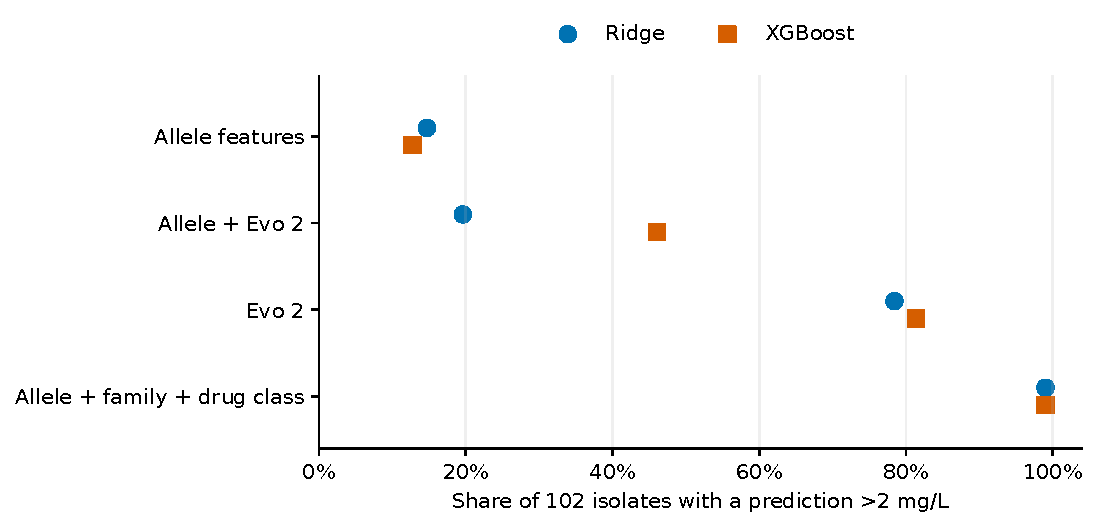
\includegraphics[width=0.9\linewidth,height=\textheight,keepaspectratio,alt={Figure 2. Exploratory external comparison on 102 highly resistant carriers of absent or rare variants. Points show the share of isolates with ceftriaxone MIC \textgreater64 mg/L whose rounded prediction exceeded 2 mg/L. The subset and family-feature analysis were motivated by the locked external errors. Points are descriptive subgroup proportions; no intervals were estimated for this exploratory read-out. ``Evo 2'' uses embeddings of annotation-selected loci.}]{figures/figure2_external_variants.pdf}
\caption{Exploratory external comparison on 102 highly
resistant carriers of absent or rare variants. Points show the share of
isolates with ceftriaxone MIC \textgreater64 mg/L whose rounded
prediction exceeded 2 mg/L. The subset and family-feature analysis were
motivated by the locked external errors. Points are descriptive subgroup
proportions; no intervals were estimated for this exploratory read-out.
``Evo 2'' uses embeddings of annotation-selected loci.}
\end{figure}

Across all external ceftriaxone rows, the family-feature XGBoost model
reached EA 0.854 (0.784--0.892), a paired increase of 0.257
(0.138--0.346) over the allele model. Family ridge reached 0.771
(0.666--0.817), an increase of 0.092 (0.034--0.145). The paired
differences come from the original reported comparisons; their last
decimal can differ from subtraction of rounded point estimates. Family
XGBoost also reached EA 0.938 for ciprofloxacin and 0.901 for
gentamicin; the paired changes were 0.005 (\ensuremath{-}0.004 to 0.012) and 0.025
(0.014--0.048), respectively. These findings describe an exploratory
reuse of the external set and do not revise the original locked verdict.

\subsection{Withholding CTX-M alleles favored curated features over Evo
2}\label{withholding-ctx-m-alleles-favored-curated-features-over-evo-2}

We next specified an experiment in which every development isolate
carrying a target allele was withheld from training. The primary targets
were the four eligible CTX-M alleles with at least 30 carriers in the
human-clinical ceftriaxone population: blaCTX-M-15, -27, -14, and -55.
Models were trained on the remaining isolates, including model selection
within their grouped development folds. This tested absence of an allele
from supervised training within the development population.

Across the four targets, there were 568 above-panel target--isolate
observations from 565 unique isolates in 45 lineage groups. An isolate
carrying more than one target contributes once in each corresponding
experiment. Paired comparisons resampled whole lineages, retaining the
observations belonging to each sampled lineage.

Curated-family models exceeded Evo 2 alone by 0.046 (0.023--0.121) for
ridge and 0.111 (0.074--0.221) for XGBoost in the share of above-panel
observations placed above 2 mg/L. Both met the stated non-inferiority
margin of \ensuremath{-}0.05, and both intervals were also entirely positive.
Differences from allele-only features were 0.915 (0.836--0.943) and
0.963 (0.916--0.981). These hypotheses were specified before the
withholding experiment, after the exploratory external analysis.

Per target and learner, family-feature models placed 97.2--100\% of
above-panel CTX-M carriers above the descriptive threshold, compared
with 85.9--100\% for Evo 2 alone and 2.2--11.1\% for allele-only models
(Figure 3). EA over all held-out CTX-M carriers ranged from 0.74 to 0.95
for family features, 0.44 to 0.87 for Evo 2, and 0.00 to 0.08 for allele
features. Thus, the family representation improved both the
threshold-side comparison and MIC agreement.

\begin{figure}
\centering
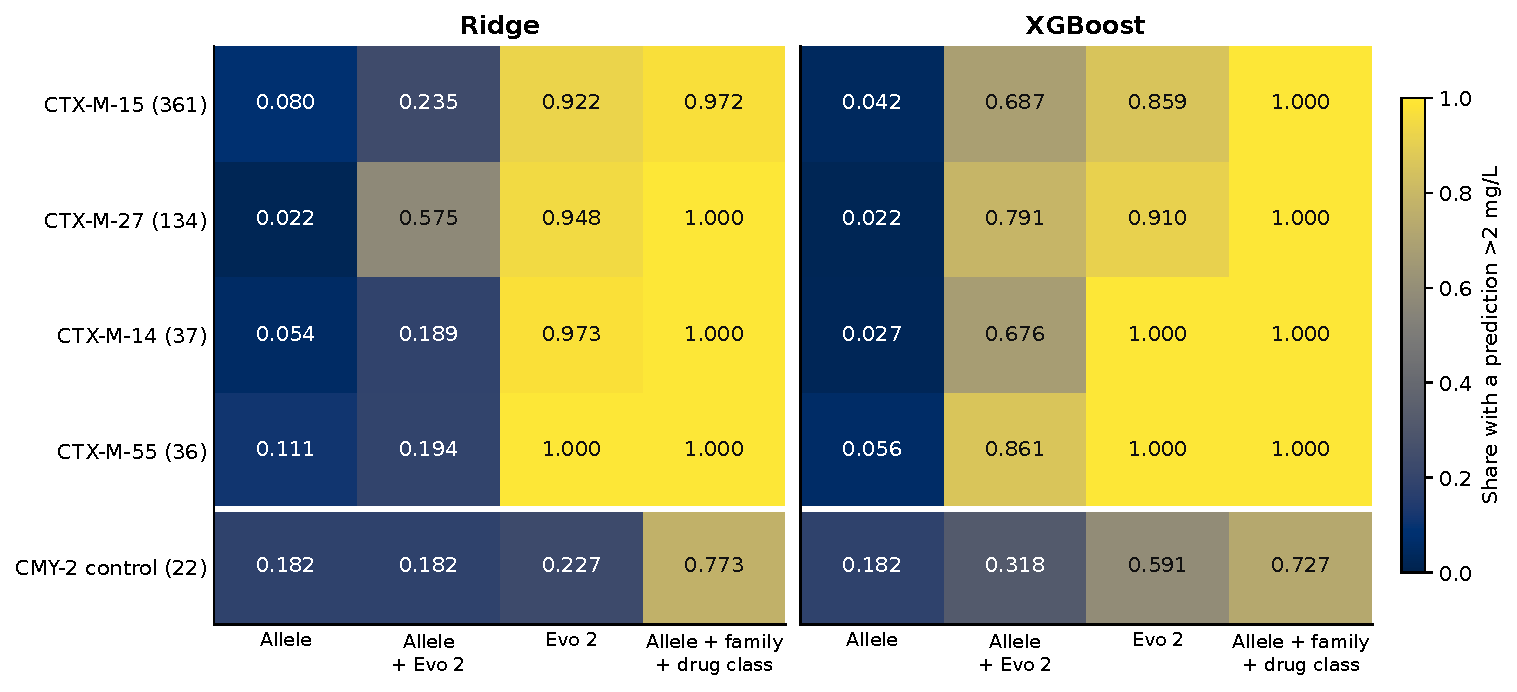
\includegraphics[width=1\linewidth,height=\textheight,keepaspectratio,alt={Figure 3. Controlled withholding of resistance alleles from development training. Each cell gives the proportion of above-panel carriers placed above the descriptive 2 mg/L threshold; panels separate ridge and XGBoost. The first four rows are the primary CTX-M targets. CMY-2 is a control without another sufficiently represented CMY allele in training. Numbers beside targets are above-panel target--isolate observations. Values are reproduced at the three-decimal precision of the report.}]{figures/figure3_leave_variant_out.pdf}
\caption{Controlled withholding of resistance alleles from
development training. Each cell gives the proportion of above-panel
carriers placed above the descriptive 2 mg/L threshold; panels separate
ridge and XGBoost. The first four rows are the primary CTX-M targets.
CMY-2 is a control without another sufficiently represented CMY allele
in training. Numbers beside targets are above-panel target--isolate
observations. Values are reproduced at the three-decimal precision of
the report.}
\end{figure}

The CMY-2 control had no other CMY allele represented by at least five
training isolates. Here, the hierarchical representation could transfer
through its drug-class indicators, but not a sufficiently represented
CMY family indicator. The above-threshold share was 0.773/0.727 for
family features, 0.227/0.591 for Evo 2, and 0.182/0.182 for allele
features (ridge/XGBoost). The descriptive OXA-1 target produced a share
of 0.994 for every model; co-carried CTX-M-15 remained in training.

Combining allele features with Evo 2 did not preserve the generalization
of embeddings alone: the above-threshold share across primary CTX-M
targets ranged from 0.189 to 0.861. This behavior is consistent with the
combined predictors relying on familiar allele indicators and
transferring less effectively when the withheld allele was absent from
their feature vocabulary. The experiment does not establish a causal
account of the fitted model's internal decision process.

\section{Discussion}\label{discussion}

The central result is that curated gene-family and drug-class features
outperformed the tested Evo 2 representation when resistance alleles
were absent from supervised training. Evo 2 recovered useful
relationships that allele-only indicators missed, but biological
grouping recovered these relationships more reliably in the controlled
withholding experiment. The exploratory external analysis showed the
same ordering on a selected set of unfamiliar, highly resistant
variants.

This finding changes how a foundation-model comparison should be
interpreted. The relevant baseline is the biological information
available to the task, including connections among alleles.
AMRFinderPlus already supplies curated functional classes
(\citeproc{ref-feldgarden2021}{Feldgarden et al. 2021}). Ignoring those
classes can make a sequence representation look more useful than a
stronger catalogue representation. Our hierarchical model retained
allele indicators and added family and class indicators, so its
advantage should be attributed to that combined representation; the
experiment does not separately estimate the effects of family pooling
and drug-class annotations.

The locked evaluation also illustrates the limits of development gains.
Lineage grouping prevented closely related isolates from being spread
across development folds, yet did not remove source associations. One
BioProject contributed approximately 73\%, 54\%, and 62\% of primary
development rows for ceftriaxone, ciprofloxacin, and gentamicin,
respectively. Another project accounted for the observed gentamicin
embedding advantage. Source-exclusion summaries and the independent
Japanese evaluation showed that this advantage did not persist. This
complements evidence that bacterial sampling structure can confound
machine learning (\citeproc{ref-yu2025}{Yu et al. 2025}), while
demonstrating why a lineage-aware split alone cannot address laboratory
or collection effects.

Several limits define the scope of the conclusion. First, the endpoint
was quantitative MIC prediction. Missing source-level assay and
interpretation metadata prevented validation of the secondary
susceptible/intermediate/resistant endpoint. The descriptive 2 mg/L
threshold in the ceftriaxone analyses is an analysis read-out, and its
above-threshold share is not a clinically validated sensitivity
estimate. EA against a censored reference is also permissive: it
measures consistency with the observed bound and cannot recover the
unmeasured MIC. Exact-reference and censoring-stratified analyses are
therefore relevant alongside the aggregate score.

Second, the external collection was resistance-enriched and filtered for
putative genomic duplicates against development. It was tested in one
central laboratory, and collection hospital identifiers were unavailable
at isolate level in the public files used here. Its performance does not
estimate routine deployment accuracy. Development methods were
heterogeneous and largely unlabelled, and source-level concentrations
restrict the diversity represented by the nominal isolate count.

Third, the family analysis was prompted by external outcomes. Locking
its new predictions before rescoring preserved its audit trail, but did
not make its design independent of that external set. The withholding
experiment supplies a controlled test inside development, with
hypotheses fixed before its own runs; it is not a second geographic
replication. It withholds allele carriers, not every lineage related to
them, and therefore isolates allele transfer under the remaining
development distribution. A fresh external cohort would be needed to
confirm family-model performance outside these data.

Fourth, our Evo 2 comparison concerns frozen 20-billion-parameter
embeddings of selected resistance loci, with mean pooling and principal
component reduction. Acquired loci were located with AMRFinderPlus, so
the embedding-only predictor still depended on curated annotations for
sequence selection. Chromosomal reference loci and acquired-unit counts
also supplied task-specific structure. These results do not address
every use of Evo 2, full-genome representations, or fine-tuning.
Pretraining-overlap analysis found near-identical matches for 14,482 of
22,767 unique acquired units (63.6\%) in the audited IMG/PR component.
This is exposure to sequence, not demonstrated exposure to MIC labels,
and it limits claims that the sequence model encountered wholly novel
determinants.

Finally, the reported bootstrap intervals quantify sampling variation
across lineage groups conditional on the fitted predictions and selected
design. They do not capture every uncertainty from training, design
adaptation, or study selection. The development rule for crediting Evo 2
was set after some development outcomes were known. No claim of a
prospectively registered study is made.

For the completed experiments, curated hierarchy was the more effective
way to transfer knowledge between related resistance variants. The
practical lesson is to include biological grouping among the baselines
used to assess genomic foundation models, and to examine source and
allele shift separately from aggregate development performance.

\section{Methods}\label{methods}

\subsection{Sources, normalization, and cohort
membership}\label{sources-normalization-and-cohort-membership}

We used frozen NCBI quantitative susceptibility and isolate snapshots
and the JARBS supplementary dataset linked to BioProject PRJDB10842
(\citeproc{ref-kayama2023}{Kayama et al. 2023}). The parent sets
comprised 10,334 development and 3,159 external isolates. Registered
assemblies were used where available; 348 development isolates and the
3,159 external isolates were assembled from linked reads in the project
workflow. The recorded genome-analysis run covered all 13,493
assemblies.

Only quantitative MIC measurements in compatible concentration units
entered the primary endpoint. Disk diffusion rows were excluded. Values
were expressed on a log2 mg/L scale; conventional labels were snapped to
a doubling dilution when within 0.1 log2 units, and off-scale values
were excluded. Repeated measurements for an isolate and antibiotic were
reconciled by intersection of their reported intervals. Conflicting or
unrepresentable intersections were excluded with a reason. Missing
metadata remained missing.

The final cohort build was 64948707. Its counts supersede intermediate
cohort versions. Human-clinical development membership required source
\texttt{epi\_type} of clinical and a human host; clinical animal
isolates were not included in that primary population. JARBS
human-clinical membership followed its documented sampling design.
Specimen source was not used as a proxy for clinical indication. The
final totals are given in Table 1; detailed source and job records
accompany the draft.

\subsection{Genome quality, grouping, and exclusion of
duplicates}\label{genome-quality-grouping-and-exclusion-of-duplicates}

The implemented assembly filters required total length 4.0--6.5 Mb, at
most 500 contigs, N50 of at least 20 kb, and at most 1,000 ambiguous
bases per 100 kb. A skani comparison with the frozen \emph{E. coli}
reference GCF\_003697165.2 required ANI of at least 95\% and alignment
of at least 50\% of the query. This species check does not distinguish
\emph{Shigella} within the \emph{E. coli} genomic boundary and is not a
comprehensive contamination assay.

Lineage groups connected Achtman sequence types differing at one of
seven MLST loci. Development split units joined those lineage groups
with genomic clusters and identifier-based duplicate groups. Genomic
clusters used ANI \ensuremath{\geq}99.9\% and minimum reciprocal aligned fraction \ensuremath{\geq}0.90.
External exclusion used the stricter putative-duplicate rule of ANI
\ensuremath{\geq}99.99\% and minimum reciprocal aligned fraction \ensuremath{\geq}0.95 against
development; shared lineage membership alone did not exclude an isolate.
Both thresholds predated model evaluation.

The initial MLST run used a mismatched scheme name and was voided.
Retyping used \texttt{ecoli\_achtman\_4} with the specified seven loci
before the final cohort and model runs. This correction did not involve
selecting a grouping using model performance.

\subsection{Catalogue and hierarchical
features}\label{catalogue-and-hierarchical-features}

AMRFinderPlus version 4.2.7 and database release 2026-08-07.1 supplied
detected AMR determinants. Allele features encoded presence of eligible
AMR gene or mutation symbols. Binary features were retained only when
present in at least five isolates in the corresponding training
partition, including during inner model selection.

The hierarchical model kept these indicators and added gene-family and
drug-subclass indicators. For beta-lactamase symbols, the final allele
number was removed, for example blaCTX-M-15 to blaCTX-M. Other gene
symbols were grouped by the implemented allele-suffix rules, for example
qnrS1 to qnrS and aac(3)-IId to aac(3)-II. Point mutations were not
pooled. AMRFinderPlus subclass labels were split into separate
indicators when multiple subclasses were listed. The same training-only
frequency filter applied to the added features.

\subsection{Evo 2 representations}\label{evo-2-representations}

We used the frozen \texttt{evo2\_20b} checkpoint through the Evo 2
implementation (\citeproc{ref-brixi2026}{{Brixi et al.} 2026};
\citeproc{ref-evo2software}{Arc Institute 2026}). Sequence units
comprised 12 reference chromosomal loci---gyrA, gyrB, parC, parE, marR,
acrR, soxR, ampC, ompF, ompC, ompR, and envZ---with 300 bp upstream, and
AMRFinderPlus-located gene units with 500 bp flanks. Reference panel
hits required at least 80\% identity over 90\% of the reference unit;
absent hits were recorded as missing. The operational acquired-unit set
includes some intrinsic AMR-labelled genes, so its name is not evidence
of horizontal acquisition for every unit.

Extraction yielded 287,069 unit rows from 13,399 eligible genomes,
deduplicated to 31,938 unique sequences containing 56.3 Mb. For each
unique sequence, token embeddings were averaged separately on both
strands and then averaged between strands. Candidate representations
came from \texttt{blocks.6.mlp.l3}, \texttt{blocks.12.mlp.l3}, and
\texttt{blocks.17.mlp.l3}. Layer selection used training folds only.

Each chromosomal locus was reduced to up to 16 principal components.
Acquired-unit vectors were averaged within an isolate and reduced to up
to 32 components, with a unit count included. Missing panel loci
contributed zero coordinates and a missingness indicator. Every
principal component analysis was refitted on the corresponding training
partition. Embedding extraction read sequences without phenotype
information; downstream transformations and learner selection used
development data. The production record reports four H100 tasks and
approximately 3.6 GPU-hours for embedding extraction; this is not the
total study compute cost.

\subsection{Learners and model
selection}\label{learners-and-model-selection}

Ridge modelled latent log2 MIC as a normal distribution with mean given
by an intercept and linear feature effects. Coefficients received an L2
penalty; the intercept and residual scale were unpenalized. For an
allowed reference dilution set with endpoints L and U, the likelihood
used the latent interval (L\ensuremath{-}1, U{]}, with infinite endpoints retained.
Optimization used L-BFGS-B. The final penalty grid ranged from 0.001 to
1,000 in powers of ten. Residual standard deviation was bounded between
0.05 and 64 log2 units following a numerical-overflow diagnosis in
development.

XGBoost used the normal accelerated failure time objective, which
accepts lower and upper response bounds
(\citeproc{ref-xgboostaft}{XGBoost Developers 2026}). Bounds were
supplied on the concentration scale. The grid crossed maximum depths 2,
3, and 4 with 100 or 300 trees; learning rate was 0.05, minimum child
weight 5, and distribution scale 1.0 in natural-log units. No external
outcome guided parameter choice.

Development performance used five frozen outer folds and four grouped
inner folds within each outer training partition. Vocabulary filtering,
dimensional reduction, layer choice, and learner hyperparameters were
fitted or selected within the relevant training partitions. The purpose
of nesting was to separate model selection from the observations used to
estimate its performance (\citeproc{ref-varma2006}{Varma and Simon
2006}). For external prediction, settings were selected using the five
development folds, followed by fitting on the full eligible development
population. Both human-clinical and all-source models used the same
external rows.

\subsection{Metrics, uncertainty, and external
locking}\label{metrics-uncertainty-and-external-locking}

Let d be the integer dilution index of a measurement. An exact reference
permits \{d\}; \ensuremath{\leq}d permits all dilutions at or below d; \textless d
permits dilutions at or below d\ensuremath{-}1; \ensuremath{\geq}d permits dilutions at or above d;
and \textgreater d permits dilutions at or above d+1. Predictions were
rounded to the nearest integer dilution with half values rounded upward.
Error was the distance to the nearest allowed dilution, with EA defined
as error \ensuremath{\leq}1. Two-step under-calls and over-calls, exact-reference
results, and reference-class summaries accompanied aggregate scoring.

Confidence intervals used 2,000 percentile bootstrap draws of whole
lineage groups, with seed 20260815. Model differences were paired on
identical observations. These intervals refer to lineage resampling of
fixed predictions. The constant baseline selected the training dilution
maximizing EA; ties preferred higher exact-reference EA and then the
lower dilution. The nearest-relative baseline used the highest-ANI
eligible development relative and predicted the finite boundary of that
relative's reference set.

The external prediction stage discarded phenotype columns while loading
external rows. Sixteen prediction files---eight model configurations for
each of two training populations---were checked and SHA-256-locked
before reference attachment. Each contained 4,515 predictions. Scoring
accepted only prediction files matching the committed lock. The first
scoring attempt stopped before producing metrics because an empty
uncertainty column in a point-prediction baseline was treated as
invalid. The corrected evaluator used the same locked predictions.

\subsection{Exploratory and controlled follow-up
analyses}\label{exploratory-and-controlled-follow-up-analyses}

The family-feature analysis was specified after the external errors were
inspected. New predictions were locked before scoring, with the post-hoc
status preserved. The 102-isolate external subgroup contained
ceftriaxone \textgreater64 mg/L references and designated variants
absent or nearly absent in primary development. Its read-out was the
share of rounded predicted dilutions above log2 MIC 1, corresponding to
\textgreater2 mg/L.

The subsequent allele-withholding experiment used the 2,822
human-clinical development isolates with a ceftriaxone reference.
Eligible targets were AMRFinderPlus cephalosporinase alleles, excluding
intrinsic blaEC, with at least 30 carriers. Every target carrier was
withheld from all supervised training and model selection for that
target. Remaining development folds were used for selection, followed by
refitting and prediction of the withheld carriers. Primary pooling
covered four CTX-M targets; CMY-2 and OXA-1 served as control and
descriptive targets.

The stated hypotheses compared the pooled above-threshold share for
family versus Evo 2 features with a non-inferiority margin of \ensuremath{-}0.05, and
family versus allele features with a superiority boundary of zero. Each
required the corresponding 95\% lower bound to exceed that boundary for
both learners. Pooling used target--isolate observations and resampled
their lineages. A scoring correction allowed an isolate to occur once
per target while preserving identical predictions.

\subsection{Reproducibility}\label{reproducibility}

The repository records source hashes, cohort and split manifests,
prediction locks, run identifiers, software corrections, and analysis
protocols. The primary modelling environment recorded Python 3.11,
XGBoost 2.1.4, scikit-learn 1.8.0, SciPy 1.17.1, NumPy 2.4.2, and pandas
2.3.3. Embedding execution recorded Evo 2 0.5.5 and PyTorch 2.7.1.
Production logs report flash-attn 2.8.3 above the declared
transformer-engine support range; finite outputs and shard checksums
were verified, but numerical equivalence across environments was not
tested. The production manifests did not record a checkpoint-content
hash. The release records the subsequently recovered cache revision and
preserves the original embedding shards. Numerical convergence flags
were retained; the bounded development rerun reproduced the reported
conclusions, although some ridge fits did not formally converge.
Complete selected settings and convergence counts accompany the
supplementary tables.

For manuscript verification, we retrieved the original completed-run
artifacts, checked the 18 committed prediction locks, and reproduced all
54 archived evaluations and 438 paired comparisons, including their
recorded bootstrap intervals, from frozen predictions. An independent
scalar implementation also checked essential agreement. The withholding
read-out and external variant subgroups were reproduced. No model was
refitted or selected during this verification. Full-precision results
and verification scripts accompany the release.

\section{Data and code availability}\label{data-and-code-availability}

Development data originated from NCBI Pathogen Detection and linked
public sequence archives. External data originated from JARBS,
BioProject PRJDB10842, and the supplementary materials of Kayama and
colleagues (\citeproc{ref-kayama2023}{Kayama et al. 2023}). Analysis
code is available in the
\href{https://github.com/Sekiromike/AMR-Resistance-Gene-Detection}{AMR-Resistance-Gene-Detection
repository}. The
\href{https://github.com/Sekiromike/AMR-Resistance-Gene-Detection/releases/tag/v1.0.0}{v1.0.0
research release} provides the cohort and exclusions, frozen splits,
allele and family features, predictions, evaluation and environment
manifests, selected sequence units, frozen embeddings, manuscript
source, and SHA-256 checksums. Original code is released under the MIT
license; third-party resources retain their existing terms. Large raw
read collections and pretrained model weights are accessed through their
upstream repositories rather than redistributed.

\section{Declarations}\label{declarations}

\textbf{Author contributions:} Rushath Rajeev directed the study and is
responsible for its scientific content, interpretation, and final
manuscript.

\textbf{Funding and acknowledgements:} This research received no
funding. Computational resources were provided by UMass Unity HPC.

\textbf{Competing interests:} The author declares no competing
interests.

\textbf{Ethics:} This computational analysis reused publicly available
bacterial genomic and susceptibility records. No new sampling or
experiments involving human participants or animals were conducted.

\textbf{AI assistance:} Claude Code and Codex assisted with software,
analysis workflows, documentation, and manuscript preparation. Codex
also assisted with result verification, tables, figures, and release
preparation. These tools are acknowledged as assistance rather than
authors; responsibility for the submitted work rests with Rushath
Rajeev.

\section*{References}\label{references}
\addcontentsline{toc}{section}{References}

\protect\phantomsection\label{refs}
\begin{CSLReferences}{1}{1}
\bibitem[\citeproctext]{ref-evo2software}
Arc Institute. 2026. \emph{{Evo 2}: Inference Software and Model
Checkpoints}. \url{https://github.com/ArcInstitute/evo2}.

\bibitem[\citeproctext]{ref-brixi2026}
{Brixi, Garyk, Matthew G. Durrant, Jerome Ku, et al.} 2026. {``Genome
Modelling and Design Across All Domains of Life with {Evo 2}.''}
\emph{Nature} 652: 1349--61.
\url{https://doi.org/10.1038/s41586-026-10176-5}.

\bibitem[\citeproctext]{ref-feldgarden2021}
Feldgarden, Michael, Vyacheslav Brover, Narjol Gonzalez-Escalona, et al.
2021. {``{AMRFinderPlus} and the Reference Gene Catalog Facilitate
Examination of the Genomic Links Among Antimicrobial Resistance, Stress
Response, and Virulence.''} \emph{Scientific Reports} 11: 12728.
\url{https://doi.org/10.1038/s41598-021-91456-0}.

\bibitem[\citeproctext]{ref-kayama2023}
Kayama, Shizuo, Koji Yahara, Yo Sugawara, et al. 2023. {``National
Genomic Surveillance Integrating Standardized Quantitative
Susceptibility Testing Clarifies Antimicrobial Resistance in
{Enterobacterales}.''} \emph{Nature Communications} 14: 8046.
\url{https://doi.org/10.1038/s41467-023-43516-4}.

\bibitem[\citeproctext]{ref-moradigaravand2018}
Moradigaravand, Danesh, Martin Palm, Anne Farewell, Ville Mustonen,
Jonas Warringer, and Leopold Parts. 2018. {``Prediction of Antibiotic
Resistance in {Escherichia coli} from Large-Scale Pan-Genome Data.''}
\emph{PLOS Computational Biology} 14 (12): e1006258.
\url{https://doi.org/10.1371/journal.pcbi.1006258}.

\bibitem[\citeproctext]{ref-varma2006}
Varma, Sudhir, and Richard Simon. 2006. {``Bias in Error Estimation When
Using Cross-Validation for Model Selection.''} \emph{BMC Bioinformatics}
7: 91. \url{https://doi.org/10.1186/1471-2105-7-91}.

\bibitem[\citeproctext]{ref-xgboostaft}
XGBoost Developers. 2026. \emph{Survival Analysis with Accelerated
Failure Time}.
\url{https://xgboost.readthedocs.io/en/stable/tutorials/aft_survival_analysis.html}.

\bibitem[\citeproctext]{ref-yu2025}
Yu, Yanying, Nicole E. Wheeler, and Lars Barquist. 2025. {``Biased
Sampling Driven by Bacterial Population Structure Confounds Machine
Learning Prediction of Antimicrobial Resistance.''} \emph{PLOS Biology}
23 (12): e3003539. \url{https://doi.org/10.1371/journal.pbio.3003539}.

\end{CSLReferences}

\end{document}
